\chapter{Microservice-Infrastruktur}
\label{chap:microserviceinfrastruktur}
Bevor man mit dem Programmieren der Anwendung anfangen kann,
gilt es einiges vorzubereiten. Dieses Kapitel beschäftigt sich
mit der Microservice-Infrastruktur der Gesamtanwendung. Hier geht
es um das Aufsetzen einer agilen Infrastruktur, die den
stetigen Auslieferungsprozess der Software ermöglicht. 
In \Cref{chap:qualitaetssicherung} geht es um Methoden und Verfahren,
die die Qualität der Software sicherstellen. Erst nach der Erstellung
der Microservice-Infrastruktur sowie der Automatisierung von
Qualitätssicherungsprozessen, kann mit der Programmierung der
Anwendung begonnen werden.

Das Kapitel Microservice-Infrastruktur ist wie folgt gegliedert:
In \Cref{sec:continuousdelivery} befasst sich die Arbeit mit
dem stetigen Softwareauslieferungsprozess, bekannt als Continuous Delivery.
In \Cref{sec:monorepoundsubmodules} wird die Aufteilung der Versionsverwaltung
in einzelne Aufbewahrungsorte diskutiert. In \Cref{sec:infrastruktur}
wird die Infrastruktur der Gesamtanwendung geschildert. Hier geht es
um Technologien, die das Auslieferungsverfahren sowie die Benutzung
der Anwendung in Produktion ermöglichen. In \Cref{sec:systemdesign}
geht es um die Gestaltung der Anwendung selbst. Hier werden die einzelnen,
für die Anwendung nötigen Komponenten erörtert und definiert. Dabei
wird auf die Frage des Tech-Stacks der einzelnen Services geklärt.
In \Cref{sec:pipelinedesign} geht es um die Pipeline, also den Auslieferungsprozess
selbst. Hier werden Vorkehrungen getroffen, um diesen zu ermöglichen.

\section{Continuous Delivery}
\label{sec:continuousdelivery}
Continuous Delivery (CD ist das Verfahren, Software in einem stetigen Zyklus auszuliefern.
Neue Technologien, wie die Containervirtualiserungssoftware Docker,
die im März 2013 von dotCloud ins Leben gerufen wurde \cite{DockerAbout2014}, vereinfachen
den stetigen Softwareauslieferungsprozess enorm. So kann man in einem automatisierten
Auslieferungsprozess, Images bauen, diese testen und selbige nach erfolgreichem
Bestehen der Tests in der Produktion verwenden. Eberhard Wolff schreibt über das Ziel von Docker in
seinem Buch "Continuous Delivery" folgendes: "Das Ziel von Docker ist es, Container für die
Distribution von Software zu nutzen. Im Vergleich zu normalen Prozessen trennen Linux-Container
einzelne Anwendungen viel besser voneinander, wenn es darum geht, die Software auf einem anderen
System zu installieren. Docker bietet ein Repository für Images an, so dass eine Vielzahl
von Servern mit identischen Images betrieben werden können."\cite[S. 56]{ContinuousDeliveryWolff}
Somit kann sichergestellt werden, dass die Software und deren Umgebung in der Testphase
sowie in Produktion die selbe ist. Immer mehr Anbieter stellen CI-Werkzeuge zur Verfügung,
die es ermöglichen eine CI/CD-Pipeline anhand von Konfigurationsdateien aufzuziehen. So bieten nun
neben Travis CI, CircleCI und Jenkins auch Versionsverwaltungshosts wie Github und
Gitlab CI-Werkzeuge zur Verfügung.\footnote{Github bietet seit 13. November 2019 eigene CI/CD-Werkzeuge an \cite{GithubCIToolsHeise}}
Vorteile eines CD-Ansatzes sind schnelle Feature-Auslieferung und somit schnellere Resonanz der Benutzer auf die Features,
Robustheit der Software durch stetiges Ausführen automatisierter Tests in der Pipeline, einfaches Zurückrollen
der Version der Anwendung in Produktion sowie einfaches Reproduzieren von Fehlern. Ein Nachteil eines CI/CD-Ansatzes ist
der große Aufwand des initialen Aufbaus der automatisierten Prozesse. Bei komplexen Änderungen des Systems müssen zudem
große Teile des automatisierten Prozesses angepasst werden.

In der Arbeit wird für die Versionsverwaltung und die stetige Softwareauslieferung ein eigener Linux-Server verwendet,
auf dem die Community Version von Gitlab installiert ist. Auf dem Linux-Server befinden sich auch eine eigene Docker
Registry sowie ein eigener Gitlab Runner\footnote{Gitlab Runner dienen zur Ausführung der Pipeline}. Der Aufbau
wird in \Cref{sec:infrastruktur} nochmal genauer behandelt. 

\section{Monorepo und Submodules}
\label{sec:monorepoundsubmodules}
In diesem Abschnitt geht es um die Aufteilung des Programmcodes in Repositories. Für die Versionsverwaltung
wird Git verwendet. Die Arbeit entscheidet sich dazu, die einzelnen Microservices in einer Monorepo unterzubringen.
Unter Monorepo versteht man die Strategie, den Programmcode aus mehreren Anwendungen, Services, Bibliotheken und Frameworks
in einer Repository unterzubringen.\cite{MonorepoTrunkBasedDevelopment} Diese Strategie verringert nicht nur den Aufwand
des Aufsetzens mehrerer Repositories, sondern gibt den Entwicklern auch einen besseren Überblick über die einzelnen
Projekte. Gerade im Fall von Microservices hat dieser Ansatz den Vorteil, dass man Änderungen in mehreren Services,
die miteinander verkoppelt sind, in einem Commit in die Versionsverwaltung einchecken kann. Dies kann verbindlich sein,
wenn Tests der Pipeline auf bestimmte Versionen der unterschiedlichen Services angewiesen sind. Verändert man beispielsweise
eine API eines Services, kann man gleichzeitig das Frontend anpassen. Die Diagramme eines Dashboards sollen allerdings
auch extern entwickelbar sein. Um dies zu ermöglichen, verwendet die Arbeit Git-Submodules.\cite{GitsubmodulesGitSCM} Mithilfe dieser Submodules
kann man andere Repositories in ein Repository integrieren. Somit können externe Entwickler das Repository des
Submodules gabeln\footnote{Unter "gabeln" oder auch "forken" versteht man das Erstellen einer eigenen Kopie eines Repositories, mit der unabhängig von der Versionierung der gegabelten Repository entwickelt werden kann.},
um in ihrem eigenen Repository Diagramme für die Anwendung zu entwickeln.

\section{Infrastruktur}
\label{sec:infrastruktur}
Wie in \Cref{sec:continuousdelivery} bereits angesprochen, beinhaltet die Infrastruktur
der Arbeit einen Linux-Server, auf welchem Gitlab CE, Gitlab Runner und eine Docker Registry
installiert sind. Desweiteren benötigt es weitere Server, für die Testphase sowie für
die Produktion. Die einzelnen Services werden einfachheitshalber mithilfe von Docker-Compose
auf einem einzelnen Server ausgeführt. Das Ziel für die Zukunft ist es, die einzelnen
Services auf einzelne Linux-Server zu verteilen. Dies soll mithilfe des Open Source IAC-Werkzeugs\footnote{IAC steht für Infrastructure as Code}
Terraform über eine Cloudanbieter-API und dem Orchestrierungssystem Kubernetes automatisiert werden.
Die Arbeit beschränkt sich allerdings auf drei Linux-Server. Einen für die Versionsverwaltung
und den CI/CD-Prozess, einen für die Testphase sowie einen für die Produktion. 
Die drei Server werden von Hetzner, einem Cloudanbieter, bereitgestellt und haben Ubuntu 18.04
vorinstalliert.\footnote{Die 3 Linuxserver haben 4 VCPUs, 16GB RAM und 160GB SSD-Speicher} 
Neben den Servern benötigt es noch Volumes, um die Daten der Datenbanken zu persistieren.
Die an die Server angebrachten Volumes werden mithilfe von Docker-Compose auf die für die
Beständigkeit relevanten Ordner der Datenbank-Container zugewiesen. Die Zuweisung variiert
je nach Datenbank. Um die Server über das Internet zu erreichen, benötigt es diverse Domains
und Subdomains, die mithilfe von DNS-Records auf die vom Server bereitgestellten
IPv4- und IPv6-Adressen verweisen.\footnote{Man kann die Server natürlich auch direkt über die IP-Adresse ansprechen.}

Die Domain "blicc.org" dient als Hauptdomain und wird in der Produktion verwendet. Der Name Blicc
wurde zur representation des Produktes gewählt. Bei einer Verwendung der Anwendung als White-Label-Produkt
wird der Name durch den der zu repräsentierenden Firma ersetzt. Der Name Blicc ist eine
veränderte Form des deutschen Wortes "Blick". Der Name wurde daher verändert, da die Verfügbarkeit
von "Blick" in den meisten Domainvariationen nicht mehr erhältlich war und zudem
überteuert angeboten wurde. Die Domain für den Server der Testphase ist "testing-stage.org".
Die beiden Domains besitzten die Subdomains "api" und "delivery". Die Subdomain "api" verweist
auf die Resource Management API; die Subdomain "delivery" verweist auf die Data Delivery API.
Desweiteren gibt es die "monitor" Subdomain, welche auf die Kontrollübersicht von Traefik
verweist. Traefik dient als Reverse-Proxy und Load-Balancer, bietet zusätzlich allerdings
auch noch geringe Überwachungsfunktionalitäten in einem webbasierten Dashboard an.
Dazu mehr in \Cref{sec:reverseproxyundloadbalancer}.

Die Docker Registry ist unter der Domain "registry.thiloilg.com", Gitlab CE
unter "gitlab.thiloilg.com" erreichbar. Die Repositories werden alle zusätzlich
auf Github.com gespiegelt. Github.com dient als drittes Backup, falls die Repositories auf dem
eigenen Gitlab Server und dem lokale Rechner verloren gehen. Mit dem Git-Befehl in
Quellcode \ref{lst:gitalias} kann man sich einen Alias setzen, um zu allen Remote Repositories
gleichzeitig zu pushen. Der senkrechte Strich im Linux Terminal, bekannt als "Pipe", trennt zwei Befehle in der
Kommandozeile. Das Ergebnis des ersten Befehls wird an den zweiten Befehl weitergereicht.

\begin{listing}
    \inputminted{sh}{snippets/sh/pushall.sh}
    \caption{Konfiguration eines eigenen Git Alias}
    \label{lst:gitalias}
\end{listing}

Für das Aufsetzen der Server benötigt man drei Schritte.
Als erstes verbindet man sich über SSH zu dem Server und richtet den die UFW
ein.\footnote{UFW steht für Uncomplicated Firewall} Dabei öffnet man alle Ports,
die von den Anwendungen des Server benötigt werden. In der Regel sind das Port 80
für HTTP und Port 443 für HTTPS. Aufgrunddessen, dass bei dem Gitlab CE Server
Port 22 bereits für die SSH verbindung benötigt wird, musste der Gitlab Shell SSH
Port auf 2222 verlegt werden. Als zweiten Schritt Installiert man alle nötigen
Programme auf dem Server. Das wichtigste der Programme ist Docker CE. In Schritt
drei kopiert man mithilfe von SCP die \code{docker-compose.yml} Datei auf den
Server und startet sie mit \code{docker-compose up}. In der Docker-Compose Datei
stehen alle wichtigen Informationen, um ein kleines Docker-Cluster aufzuziehen.
Bei dem Server für die Testphase sowie dem Produktionsserver ist dieser Prozess
in der Gitlab CI Pipeline automatisiert. Eine genauere Beschreibung der
Pipeline befindet sich in \Cref{sec:pipelinedesign}.

\section{Systemdesign}
\label{sec:systemdesign}
In diesem Abschnitt wird das Grundkonzept aus \Cref{subsec:trennungvonlogic}
über die Trennung von logic weiter ausgebaut und daraus ein komplettes System
entwickelt. Dabei wird auch die Frage nach den verschiedenen Technologien für
die Services geklärt. 

% Wahl der Technologien, Tech-Stack?
% Anforderungen an die Technologien
% Umfeld etc
% Geschwindigkeit der Entwicklung
\begin{figure}
    \label{figure:microserviceinfrastruktur}
    \begin{center}
    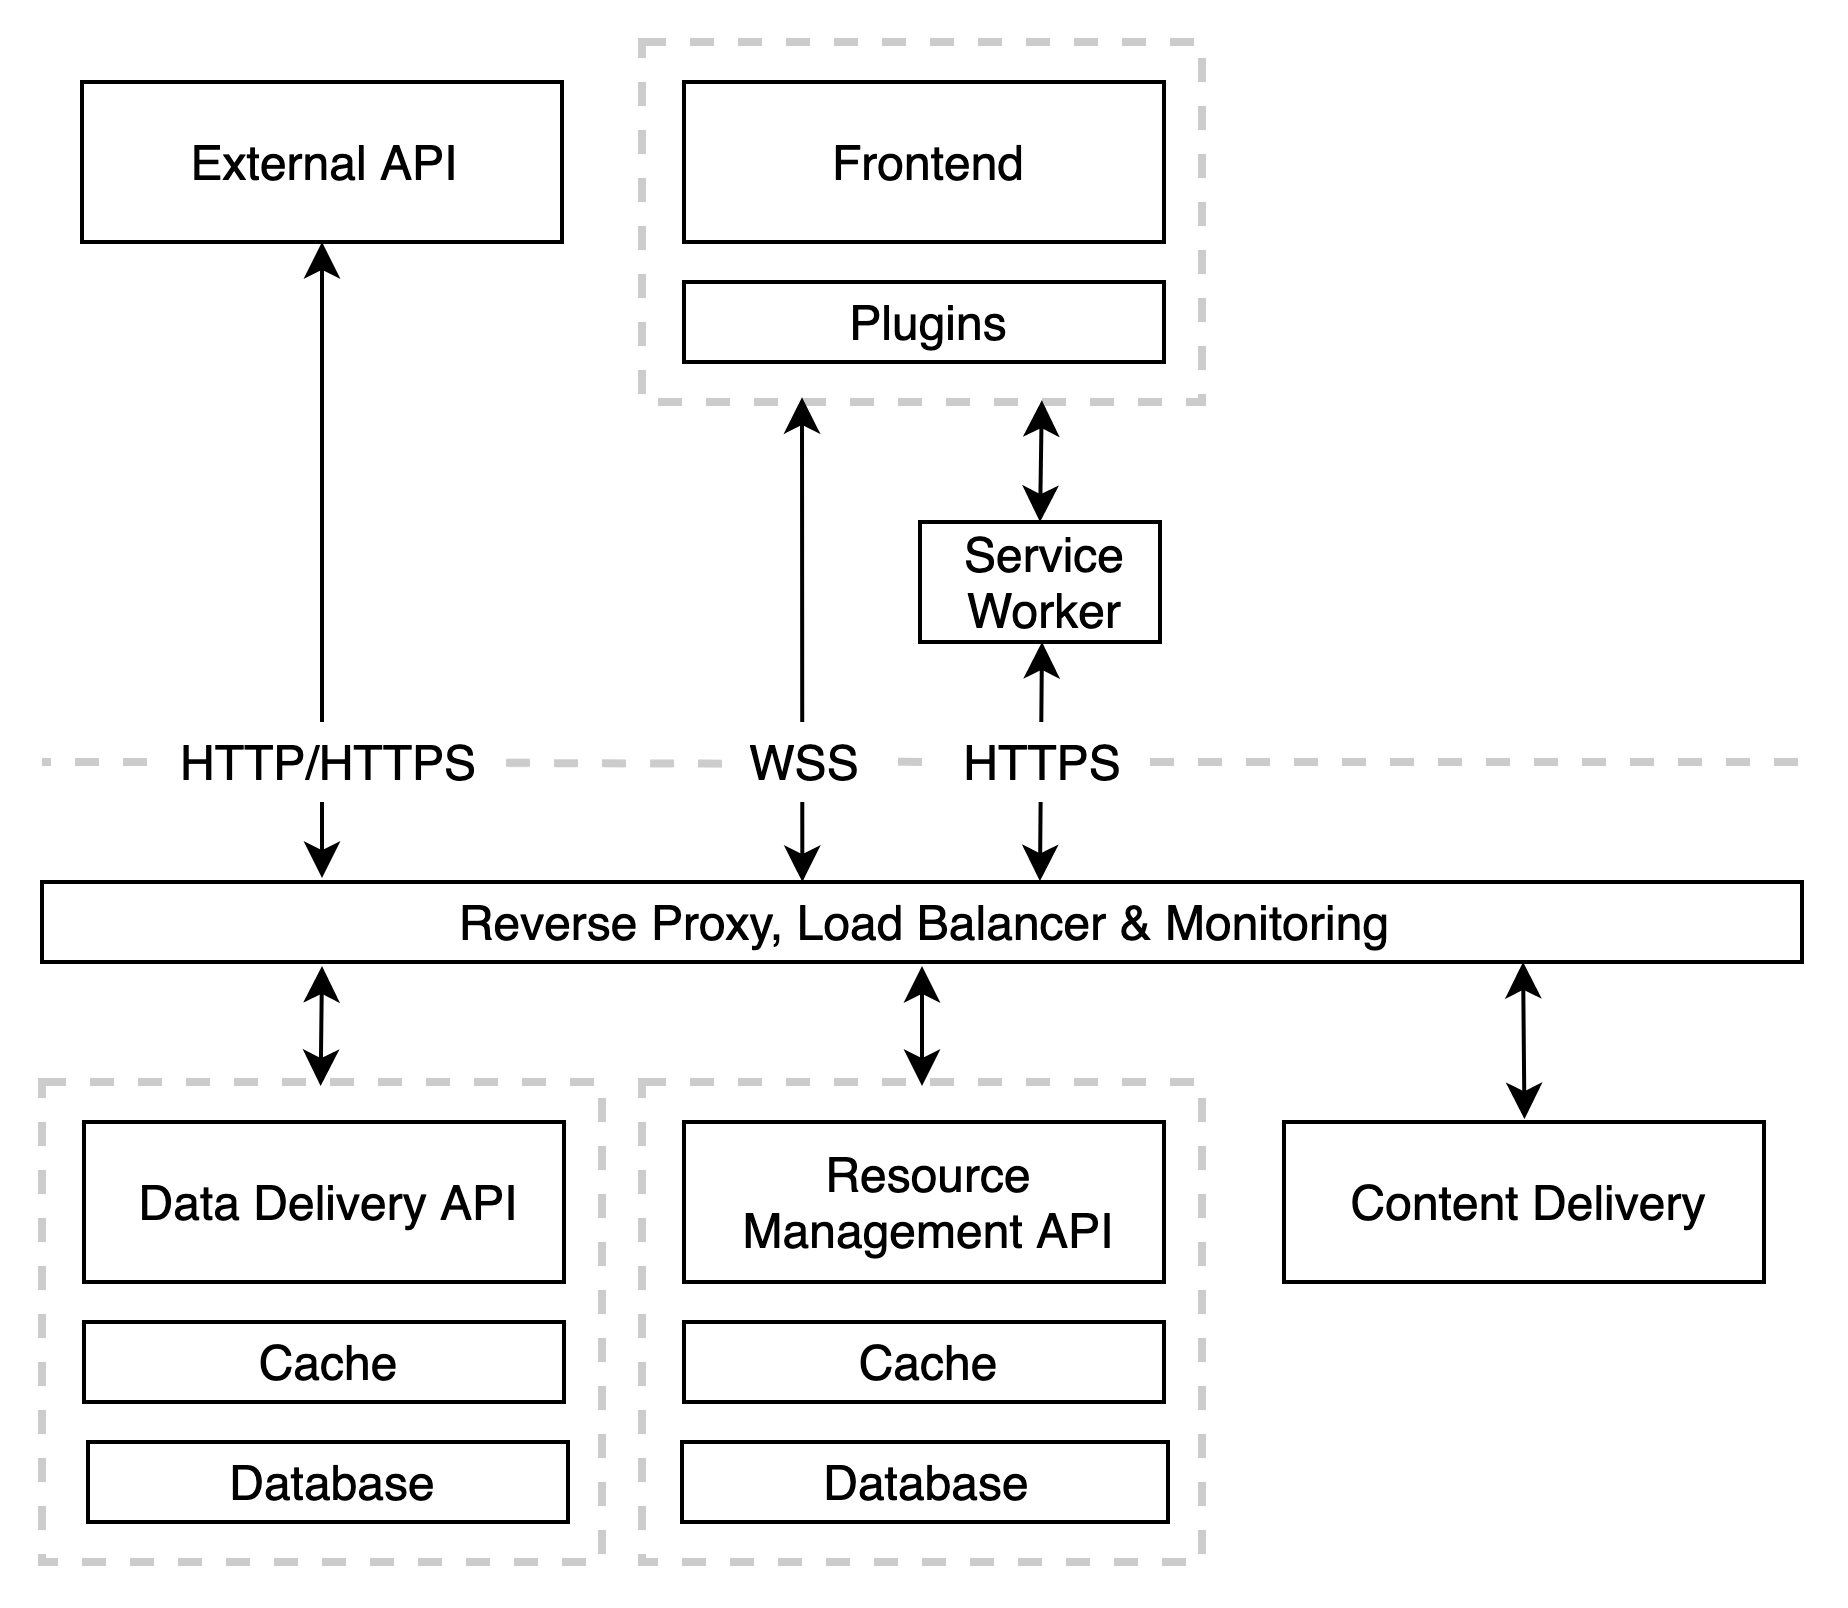
\includegraphics[scale=0.2]{img/abbildungen/MicroserviceInfrastruktur}
    \end{center}
    \caption{Übersicht über die Microservice-Infrastruktur}
\end{figure}

\subsection{Reverse Proxy und Load Balancer}
\label{sec:reverseproxyundloadbalancer}

Der Service läuft selbst in einem
Docker-Container und hat die primäre Aufgabe, die 

\subsection{Inhaltsauslieferung}
\label{sec:inhaltsauslieferung}

%% compression
% CDM

\subsection{Resource Management API}
\label{sec:resourcemanagementapi}

\subsection{Data Delivery API}
\label{sec:datadeliveryapi}

\subsection{Monitoring}
\label{sec:monitoring}

\subsection{Wartung}
\label{sec:wartung}
% clean up von server und docker setup

\section{Pipeline Design}
\label{sec:pipelinedesign}

\subsection{Umgebungsvariablen}
\label{subsec:umgebungsvariablen}

\subsection{Stages}
\label{subsec:stages}
% Continuous Integration mit Gitlab

% Docker Verlauf anzeigen

\subsection{Docker Compose Setup}
\label{subsec:dockercomposesetup}

\subsection{Health-Checks}
\label{subsec:healthcheck}
In Microservice-Infrastrukturen sind die einzelnen Services eng miteinander verknüpft
und voneinander abhängig. Um die Verfügbarkeit sicherzustellen, werden auf
Serviceebene Healthcheckendpunkte bereitgestellt. Diese spiegeln den aktuellen
Gesundheitszustand des jeweiligen Dienstes wieder. Ein Healthcheckendpunkt
ist speziell dann nützlich, wenn ein Dienst oder ein Verfahren von einem anderen
abhängig ist. So ist beispielsweise die Backendapi von der Datenbank
abhängig. Andererseits ist der Frontenddienst sowie das Apitestverfahren
in der Buildpipeline von der Backendapi abhängig. 

\begin{listing}
    \label{lst:healthcheck}
    \inputminted{sh}{snippets/sh/healthcheck.sh}
    \caption{Healthcheckbeispiel in der Gitlab CI}
\end{listing}

